\chapter{INTRODUÇÃO}
\label{chp:introduction}


Busca de código-fonte é uma tarefa essencial no trabalho de engenheiros e desenvolvedores de \textit{software} \cite{Rahman2018EvaluatingHD}. \textcite{Sadowski2015HowDS} mostrou que, em média, um engenheiro realiza 5 sessões de busca de código-fonte com 12 buscas por sessão, totalizando assim 60 buscas por código-fonte durante um dia de trabalho. \textcite{Xia2017WhatDD} também mostra que trechos de código-fonte estão entre os itens mais buscados pelos engenheiros de \textit{software}.

Porém, um dos problemas conhecidos da área de recuperação de informação é o \textit{term mismatch} ou \textit{vocabulary mismatch} \cite{Furnas1987TheVP} \cite{Carpineto2012ASO}. Em busca de código-fonte, esse problema se dá quando os termos da busca providos pelo usuário não coincidem com os termos utilizados nos trechos de código-fonte correspondentes \cite{Nie2016QueryEB}. Além disso, a maioria das ferramentas de busca de código-fonte atuais realizam buscas por correspondência textual. Tais buscas utilizam o termo buscado pelo usuário (tal termo também é chamado de \textit{query}) e procuram códigos-fonte que contenham este mesmo termo. Esse método de busca, no contexto de busca de código-fonte a partir de linguagem natural, tende a incorrer neste problema de \textit{term mismatch}.

Por exemplo: considere que o engenheiro de \textit{software} queira encontrar códigos-fontes relacionados ao processo de autenticação de um usuário em determinado sistema. Normalmente, tal processo é chamado de \textit{login}. Porém, há diversos outros termos que também são utilizados para o mesmo processo de autenticação, como \textit{signin}, \textit{autenticar} e outros. A figura \ref{fig:intro:login-search} mostra um exemplo de busca de código-fonte por correspondência textual, utilizando a \textit{query} \textit{login}.

\begin{figure}[H]
  \centering
  \caption{Exemplo de busca por correspondência textual}
  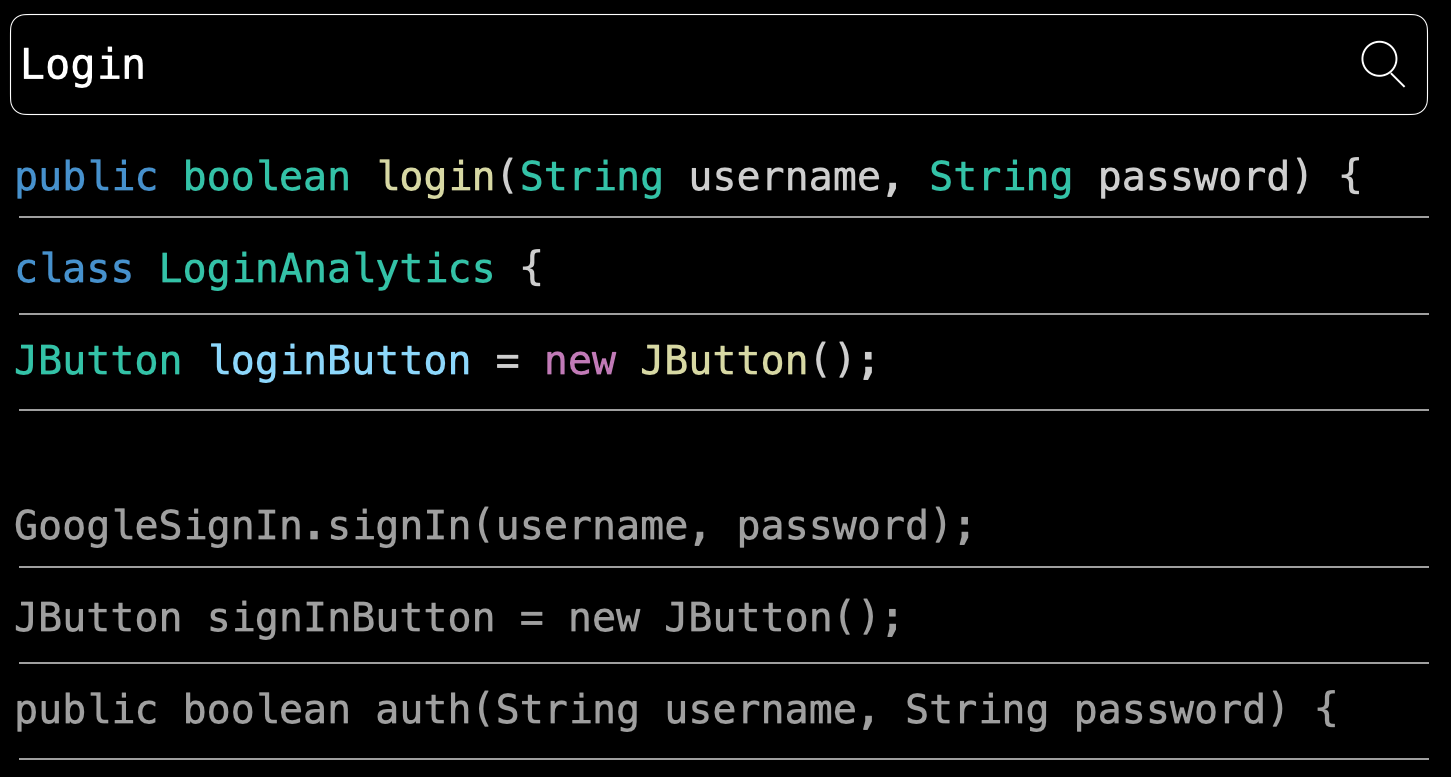
\includegraphics[width=\textwidth,keepaspectratio=true]{resources/images/introducao/login-search.png}
  \label{fig:intro:login-search}
\end{figure}

Conforme visto na figura \ref{fig:intro:login-search}, para a \textit{query} \textit{login} foram encontrados três trechos de código-fonte que continham a palavra \textit{login}. Entretanto, os três últimos trechos de código-fonte, mostrados figura \ref{fig:intro:login-search}, não foram encontrados, embora também sejam relacionados ao mesmo processo de autenticação do usuário no sistema.

Para mitigar esse problema de \textit{term mismatch} na busca de código, vem sendo aplicadas técnicas de \gls{nlp} como \textit{query expansion} \cite{Nie2016QueryEB}, modelo booleano \cite{lv2015codehow} e, mais recentemente, modelos \textit{transformers} como o \textit{CodeBERT} \cite{Feng2020CodeBERTAP}. Tais modelos \textit{transformers} se tornaram o estado da arte em busca de código-fonte utilizando linguagem natural pelo fato destes serem capazes de adicionar informações semânticas às buscas \cite{Guo2021GraphCodeBERTPC}. Isso significa que tais modelos compreendem, além das informações textuais contidas no trecho de código, informações semânticas sobre o código-fonte, como quais tarefas este realiza.

Para realizar o treinamento de tais modelos \textit{transformers}, normalmente é utilizado uma estrutura chamada par código-fonte/descrição ou par código-fonte/comentário. Tal estrutura contém tanto um trecho de código-fonte, escrito em linguagem de programação, quanto um trecho, escrito em linguagem natural, descrevendo as tarefas realizadas por tal código-fonte. Um exemplo de par código-fonte/descrição pode ser encontrado na figura \ref{fig:intro:code-description-pair}.

\begin{figure}[H]
  \centering
  \caption{Exemplo de um par código-fonte/descrição}
  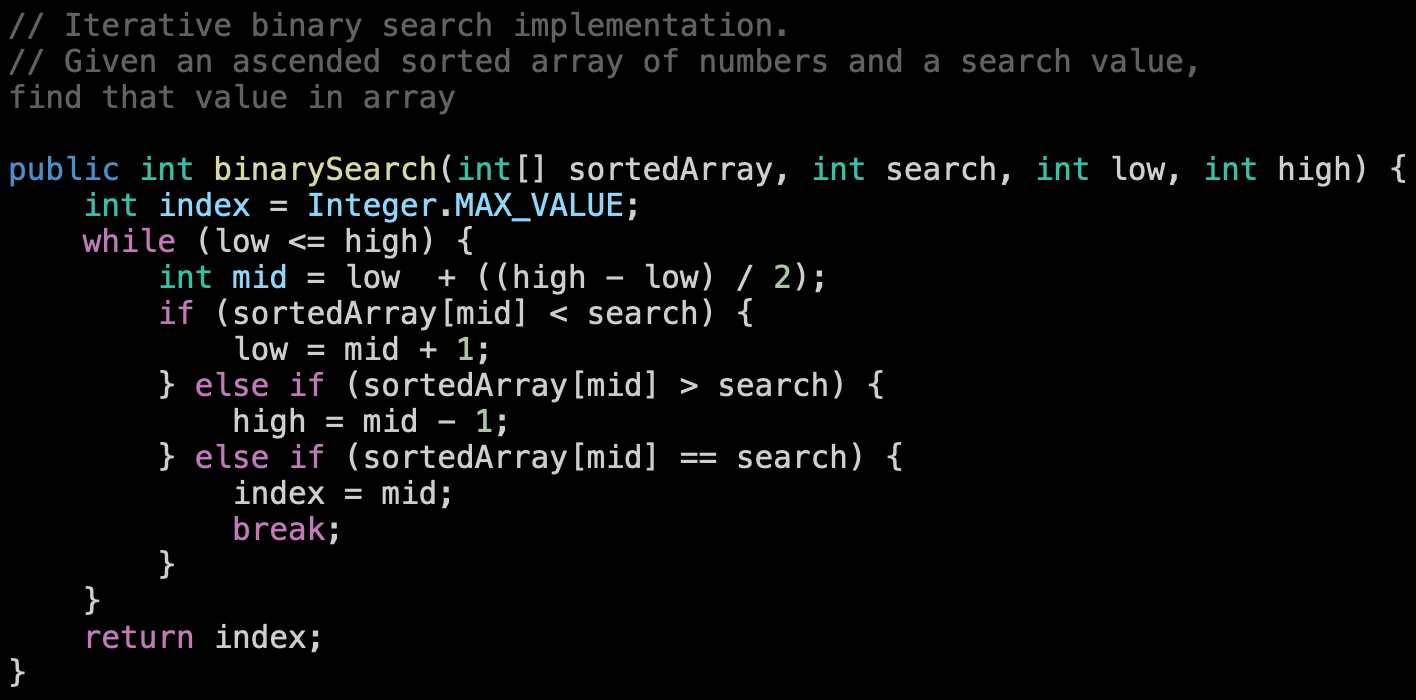
\includegraphics[width=\textwidth,keepaspectratio=true]{resources/images/introducao/code-desc-pair.png}
  \label{fig:intro:code-description-pair}
\end{figure}

Na figura \ref{fig:intro:code-description-pair}, nota-se que há um trecho de código-fonte que realiza determinadas tarefas, e outro trecho, escrito em inglês (linguagem natural), descrevendo as tarefas realizadas pelo código-fonte em questão. Com isso, observa-se que o problema de busca de código-fonte lida com dois domínios de linguagem: o primeiro é o da linguagem natural, o qual contempla tanto a descrição do código-fonte quanto os termos de busca fornecidos pelo usuário. Já o segundo domínio refere-se às linguagens de programação, nas quais são escritos os trechos de códigos-fonte que serão buscados.

Diante disso, o objetivo do presente trabalho é comparar modelos de \textit{embeddings} para recuperação de código-fonte a partir de buscas feitas em linguagem natural. Para tanto, será implementado um modelo de comparação de \textit{embeddings}, com parâmetros definidos experimentalmente conforme descrito no capítulo \ref{chp:experiments}, o qual será treinado para comparar a similaridade dos \textit{embeddings} produzidos por modelos \textit{transformers} de linguagem natural e de linguagem de programação.

\section{Objetivo}
O objetivo desse trabalho é criar e avaliar um modelo de rede neural para comparação de \textit{embeddings} gerados por redes \textit{transformers} de dois domínios diferentes: linguagem natural e linguagem de programação. 

\section{Organização do trabalho}
O presente trabalho está organizado da seguinte forma: no capítulo \ref{chp:relatedWorks} é apresentado um retrato do estado da arte das áreas que o presente trabalho abrange, como busca de código e modelos \textit{transformers}. O capítulo \ref{chp:concepts} contém os principais conceitos teóricos abordados no presente trabalho. O capítulo \ref{chp:methodology} apresenta, em detalhes, a metodologia aplicada durante o desenvolvimento do trabalho. No capítulo \ref{chp:experiments} são descritos os experimentos realizados durante o estudo.
